\section{Parallelizing $k$-CFA with LVish} \label{s:lvish-k-cfa}

\TODO{Edit this section.}

We now evaluate 
% whether the Haskell LVish implementation provides increased expressiveness while achieving speedups on
% standard hardware.  
the expressiveness and performance of our Haskell LVish implementation.
We expect LVish to particularly shine for:
  (1) parallelizing complicated algorithms on structured data that pose 
    challenges for other deterministic paradigms, and 
  (2) composing pipeline-parallel stages of computation 
     (each of which may be internally parallelized).



In this section, we focus on a case study that fits this mold:
\emph{parallelized control-flow analysis}.  We discuss the process of
porting a sequential implementation of $k$-CFA to a parallel
implementation using LVish.
%% As we will see, the LVish approach yields
%% a promising parallel speedup, even when alternative deterministic
%% parallelization approaches do not.
\ifx\fulltr\undefined
%%% Text for paper
In the companion technical
report~\cite{Freeze-TR}, 
\else
%%% Text for TR
In Appendix~\ref{app:graph-algs}),
\fi
we also give benchmarking results for LVish
implementations of two graph-algorithm microbenchmarks: breadth-first
search and maximal independent set.


% Cut for space -- LK
%% Composing multiple such microbenchmarks demonstrates the pipelining benefit:
%% especially in worst-case scenarios where one phase has limited parallelism (such
%% as BFS on a graph with long linear-chains).  LVish applications enable subsequent
%% phases of computation to begin early, whereas the reference C++/Cilk
%% implementations we compare against do not.


%% These applications are fine-grained, and handlers or blocking $\GET$ operations
%% used per-vertex incur significant overhead.  

%% In the current implementation, LVish handlers and blocking LVish $\GET$
%% operations pose too high of an overhead to achieve good absolute performance for
%% BIS or MIS.

% Cut for space -- I don't think this really belongs in the POPL paper
% (that Google URL may not persist?) but we can talk about it in the
% TR. -- LK

%% \paragraph{Open benchmarking process}
%% While we do not report all the details of our benchmarks here, 
%% the benchmarking framework itself is accessible.
%% %
%% The logs for all benchmark runs are available in a Jenkins CI
%% instance\footnote{\url{http://cs.indiana.edu/~rrnewton/jenkins},
%%   ``Benchmark\_LVish''},
%% %
%% and the data set is openly available as a Google Fusion Table\footnote{
%% % \url{https://www.google.com/fusiontables/DataSource?docid=1YxEmNpeUoGCBptDK0ddtomC_oK2IVH1f2M89IIA}
%% \url{http://goo.gl/B942Ku}
%% }, which supports browsing and plotting
%% via a web interface, and live, automatic update with new data.

% \rnote{In this section we evaluate on a single-socket Westmere-Ex
% machine.... no we're sticking with the 12 core delta for now....}

% \subsection{Control Flow Analysis: k-CFA}

\subsubsection{$k$-CFA}
%================================================================================

The {\em $k$-CFA} analyses provide a hierarchy of increasingly precise methods
to compute the flow of values to expressions in a higher-order language.  
For this case study, we began with a simple, sequential implementation of $k$-CFA 
translated to Haskell from a version by Might \cite{MightkCFABlog}.\footnote{Haskell
 port by Max Bolingbroke: \url{https://github.com/batterseapower/haskell-kata/blob/master/0CFA.hs}.}
The algorithm processes expressions written in a
continuation-passing-style $\lambda$-calculus.
It resembles a nondeterministic abstract interpreter in which
stores map addresses to {\em sets} of abstract values, and function
application entails a cartesian product between the operator and operand sets.
%
Further, an address models not just a static variable, but includes a fixed $k$-size window
of the calling history to get to that point (the $k$ in $k$-CFA).
%
Taken together, the current 
% It defines abstract system states, including a 
redex, environment, store, and call history make up the abstract state of the
program, and the goal is to explore a graph of these abstract states.  
%
%% For our monovariant analysis, the last step merely returns a
%%   stripped down mapping from variables to expressions that may flow to that
%%   variable, throwing away temporal information.
%
\new{This graph-exploration phase is followed by a second, summarization phase
that combines all the information discovered into one store.}

\paragraph{Phase 1: breadth-first exploration}

The following function
from the original, sequential version of the algorithm
expresses the heart of the search process:

%% \begin{lstlisting}
%% type Var = String
%% type Label = Int
%% data Exp = Halt | Ref Var | Lam Label [Var] Call
%% data Call = Call Label Exp [Exp]                
%% \end{lstlisting}

\begin{lstlisting}
explore :: Set State -> [State] -> Set State
explore seen [] = seen
explore seen (todo:todos)
  | todo `member` seen = explore seen todos
  | otherwise   = explore (insert todo seen)
                          (toList (next todo) ++ todos)  
\end{lstlisting}
%
This code uses idiomatic Haskell data types like @Data.Set@ and lists.
%
\new{However, it presents a dilemma with respect to exposing
  parallelism.  Consider
  attempting to parallelize \lstinline|explore| using purely functional
  parallelism with futures---for instance, using the Strategies library~\cite{marlow-par}.
  An attempt to compute the next states in parallel would 
  seem to be thwarted by
  the main thread rapidly forcing each new state to perform the
  seen-before check, \lstinline{todo `member`} \lstinline{seen}.
  %
  There is no way for independent threads to ``keep going'' further
  into the graph; rather, they check in with \lstinline{seen} after one step.
}

\new{We confirmed this prediction by adding a parallelism annotation:
\lstinline{withStrategy (parBuffer 8 rseq) (next todo)}. 
The GHC runtime
reported that 100\% of created futures were ``duds''---that is, the main
thread forced them before any helper thread could assist.  Changing
\lstinline{rseq} to \lstinline{rdeepseq} exposed a small amount of parallelism---238/5000 futures were successfully executed in parallel---yielding no actual speedup.}

\paragraph{Phase 2: summarization}

\new{The first phase of the algorithm produces a large set of states, with stores that need to be
  joined together in the summarization phase.
  When one phase of a computation produces a large data structure that is immediately processed by the next phase, lazy
  languages can often achieve a form of pipelining ``for free''.
  This outcome is most obvious with \emph{lists}, where the head element can be consumed
  before the tail is computed, offering cache-locality benefits.}
\new{Unfortunately, when processing a pure \lstinline{Set} or \lstinline{Map} in
  Haskell, such pipelining is not possible, since the data structure is internally represented by a balanced tree whose structure is not known until
  all elements are present.  Thus phase 1 and phase 2 cannot overlap in the
  purely functional version---but they will in the LVish version, as we will see.
%
  In fact, in LVish we will be able to achieve partial deforestation in addition
  to pipelining.
%
  Full deforestation in this application is impossible, because the
  \lstinline{Set}s in the implementation serve a memoization purpose: they prevent
  repeated computations as we traverse the graph of states.
}

%% Worse yet, the purely functional implementation creates many diverging copies
%% of the store, only to union them back together:
%% \begin{lstlisting}
%% summarize states = fold (\(State _ _ store' _) store ->
%%                            store `storeJoin` store') 
%%                         empty states
%% \end{lstlisting}
%% Avoiding this problem would require invasive changes to the program and would
%% still not present opportunities for parallelism.


\subsubsection{Porting to the LVish Library}
% We began\lk{we should decide whether to use past tense or not; above it's
% ``began''}
Our first step was a {\em verbatim} port to LVish.  We changed the original, purely
functional program to allocate a new LVar for each new
set or map value in the original code.
This was done simply by changing two types, @Set@ and @Map@, to their
monotonic LVar counterparts, @ISet@ and @IMap@.
\new{In particular, a store maps a program location (with context) onto a set of
  abstract values:}

%%  with LVars supporting standard @map@ and
%% @fold@-style operations isomorphic to those for the pure data structures.
%% % making it straightforward to write LVish programs in idiomatic style.

% Literally, the only change is to 

\begin{lstlisting}
  import Data.LVar.Map as IM
  import Data.LVar.Set as IS
  type Store s = IMap Addr s (ISet s Value)
\end{lstlisting}
%% type Store s = IMap Addr s (ISet s Value)
%% type Store s = IMap Addr s (Denotable s)
%% type Denotable s = ISet s Value
%
Next, we replaced allocations of containers, and @map@/@fold@ operations
over them, with the analogous operations on their LVar counterparts.
%
The @explore@ function above was replaced by the
simple graph traversal function from Section~\ref{section:intro}!  
% This allows search to proceed in parallel 
%
These changes to the program were mechanical, including converting pure
to monadic code.
Indeed, the key insight in doing the verbatim port to LVish
was to consume LVars as if they were pure
values, ignoring the fact that an LVar's contents are spread out over space and time and
are modified through effects.

In some places the style of the ported code is functional, while in others it is
imperative.  For example, the @summarize@ function uses nested @forEach@
invocations to accumulate data into a store map:
\begin{lstlisting}
  summarize :: ISet s (State s) -> Par d s (Store s)
  summarize states = do
    storeFin <- newEmptyMap
    IS.forEach states   $ \ (State _ _ store _) -> 
      IM.forEach store  $ \ key vals -> 
        IS.forEach vals $ \ elmt  -> 
          IM.modify storeFin key (putInSet elmt)
    return storeFin    
\end{lstlisting}
% $
While this code can be read in terms of traditional parallel nested loops, it in
fact creates a network of handlers that convey incremental updates from one LVar
to another, in the style of data-flow networks.  That means, in particular, that
computations in a pipeline can \emph{immediately} begin reading
results from containers (\eg, @storeFin@), long before their contents are final.

\new{The LVish version of $k$-CFA contains 11 occurrences of \lstinline{forEach}, as well
  as a few {\em cartesian-product} operations.  The cartesian products serve
  to apply functions to combinations of all possible values that arguments
  may take on, greatly increasing the number of handler events in
  circulation.  Moreover, chains of handlers registered with \lstinline{forEach}
  result in cascades of events through six or more handlers.  The runtime
  behavior of these would be difficult to reason about.  Fortunately, the
  programmer can largely ignore the temporal behavior of their program, since all
  LVish effects commute---rather like the way in which a lazy
  functional programmer typically need not think about the order in which
  thunks are forced at runtime.}

\new{Finally, there is an optimization benefit to using handlers.  Normally, to flatten a nested data structure such as
  \lstinline{[[[Int]]]} in
  a functional language, we would need to
  flatten one layer at a time and allocate a series of temporary
  structures.  
%% (Indeed, handling \lstinline{concatMap} has proved difficult for
%%   deforestation optimizations.)
  The LVish version avoids this; for example,
  in the code for \lstinline{summarize} above, 
  three \lstinline{forEach} invocations are used to traverse a
  triply-nested structure, and yet the
  side effect in the innermost handler directly updates the final accumulator,
  \lstinline{storeFin}.
}

\begin{figure}
\vspace{-4mm}
\begin{center}
  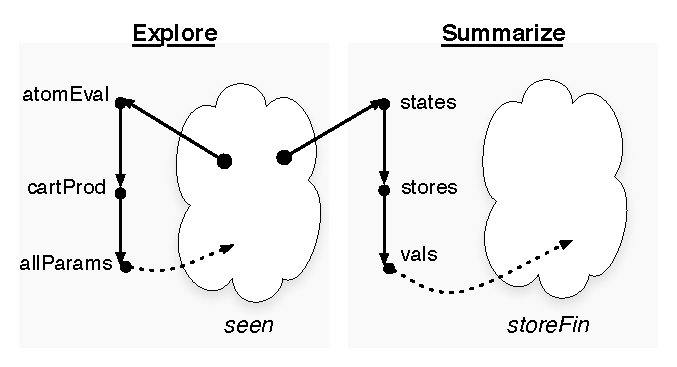
\includegraphics[width=3.1in]{chapter4/figures/DataFlowNet.pdf}
\end{center}
\vspace{-4mm}
  \caption{Simplified handler network for $k$-CFA.  Exploration and
    summarization processes are driven by the same LVar.  The triply-nested
    \lstinline{forEach} calls in \lstinline{summarize} become a chain of three handlers.}
\vspace{-4mm}
  \label{fig:dataflow}
\end{figure}


\paragraph{Flipping the switch}

%% \new{The LVish concurrent data structures have higher overhead if used only once
%%   without modification and copied repeatedly.
\new{The verbatim port uses LVars poorly: copying them repeatedly and discarding them
without modification.  This effect overwhelms the benefits of partial
deforestation and pipelining, and}
 the {\em verbatim} LVish port has a small performance overhead relative to the
 original.  But not for long!
% is a much easier starting point for overcoming the performance problems
% mentioned above.  
\new{The most clearly unnecessary operation in the verbatim port is in the
  \lstinline{next} function.}  Like the
pure code, it creates a fresh store to extend with new bindings as we take each
step through the state space graph:
\begin{lstlisting}
   store' <- IM.copy store 
\end{lstlisting}
Of course, a ``copy'' for an LVar is persistent: it is just a handler that
forces the copy to receive everything the original does.  But in LVish, it is
also trivial to {\em entangle} the parallel branches of the search, allowing them to
share information about bindings, simply by {\em not} creating a copy:
\begin{lstlisting}
   let store' = store 
\end{lstlisting}
This one-line change speeds up execution by up to $25\times$ on a single thread, and the
asynchronous, @ISet@-driven parallelism enables subsequent parallel speedup as well
(up to $202\times$ total improvement over the purely functional version).

Figure~\ref{fig:bench} shows performance data for the ``blur'' benchmark drawn
from a recent paper on $k$-CFA \cite{earl-might-icfp-2012}.  (We use $k=2$ for the
benchmarks in this section.)  In general, it proved difficult to generate
example inputs to $k$-CFA that took long enough to be candidates for parallel
speedup.  We were, however, able to ``scale up'' the blur benchmark by
replicating the code $N$ times, feeding one into the continuation argument for
the next.  Figure~\ref{fig:bench} also shows the results for one synthetic benchmark
that managed to negate the
benefits of our sharing approach, which is simply a long chain of $300$ ``not''
functions (using a CPS conversion of the Church encoding for booleans).  It has a small state space of large states with many
variables (600 states and 1211 variables).

%% Other simple attempts, however, to generate large synthetic
%% benchmarks simply wouldn't go slow enough. 

%%  (For example, we created a tree of
%% conditionals that converged very quickly).  


\paragraph{The role of lock-free data structures}
As part of our library, we provide lock-free implementations of
finite maps and sets based on concurrent skip lists~\cite{art}.\footnote{In fact,
  this project is the first to incorporate {\em any} lock-free data
  structures in Haskell, which required solving some unique problems
  pertaining to Haskell's laziness and the GHC compiler's
  assumptions regarding referential transparency.  But we lack the space to
  detail these improvements.}  We
also provide reference implementations that use a nondestructive
@Data.Set@ inside a mutable container.
% 
Our scalable implementation is not yet carefully optimized, and at one
and two cores, our lock-free $k$-CFA is $38\%$ to $43\%$ slower than the reference implementation on the ``blur'' benchmark.
% (/ 5.21 3.64) (/ 2.69 1.94)
%
But the effect of scalable data structures is quite visible on a 12-core
machine.\footnote{Intel Xeon 5660; full machine details available at \url{https://portal.futuregrid.org/hardware/delta}.}
Without them, ``blur'' (replicated $8\times$) stops scaling and begins
% and plateaus or 
slowing down slightly after four cores.  Even at four cores, variance is high in
the reference implementation (min/max $0.96$s / $1.71$s over 7 runs).  With
lock-free structures, by contrast, performance steadily improves to a speedup of
$8.14\times$ on 12 cores ($0.64$s at $67\%$ GC productivity).
Part of the benefit of LVish is to allow purely functional programs to
make use of lock-free structures, in much the same way that the \texttt{ST} monad allows
access to efficient in-place array computations.

\if 0 % sadly no space for this...
Finally, we note that other search processes can benefit from sharing
information asynchronously through a shared ``blackboard'', especially if doing
so is deterministic and easy to use, as it is with LVish.  Processes that
monotonically restrict (\eg, shrinking sets) the possibilities are also
candidates.  In the future, we plan to examine parallel logic programming in
this light.
\fi

% blurN_8 times, delta, median of 7 trials WITH -qa (which makes a difference):
% 1:  5.21  (92% productivity)
% 2:  2.69
% 4:  1.42  (3.66X speedup)   REALTIME 1.39 1.41 1.49
% 6:  1.06
% 8:  0.84
% 10: 0.75
% 12: 0.64  (67% productivity, 8.14X speedup)

%% pure-in-a-box version, min/med/max:
%% The variance is large.
% 1:  REALTIME 3.64 3.65 3.65
% 2:  REALTIME 1.92 1.94 1.95
% 4:  REALTIME 1.20 1.33 1.53
% 6:  REALTIME 1.14 1.57 1.69
% 8:  REALTIME 1.15 1.50 1.70
% 10: REALTIME 0.96 1.46 1.71
% 12: REALTIME 1.15 1.43 1.71

% (/ 3.65 1.43) 2.5x
% (/ 3.65 1.33) 2.7X

\begin{figure}  
\lk{TODO: Ryan, we should try to make this legible when printed black
  and white.}

%% This could be a bar-chart showing the 
%% parallel speedup for cfa-lvish-in place,
%% and having one "broken" bar with a 
%% number at the top for the slow original perf
\begin{center}
  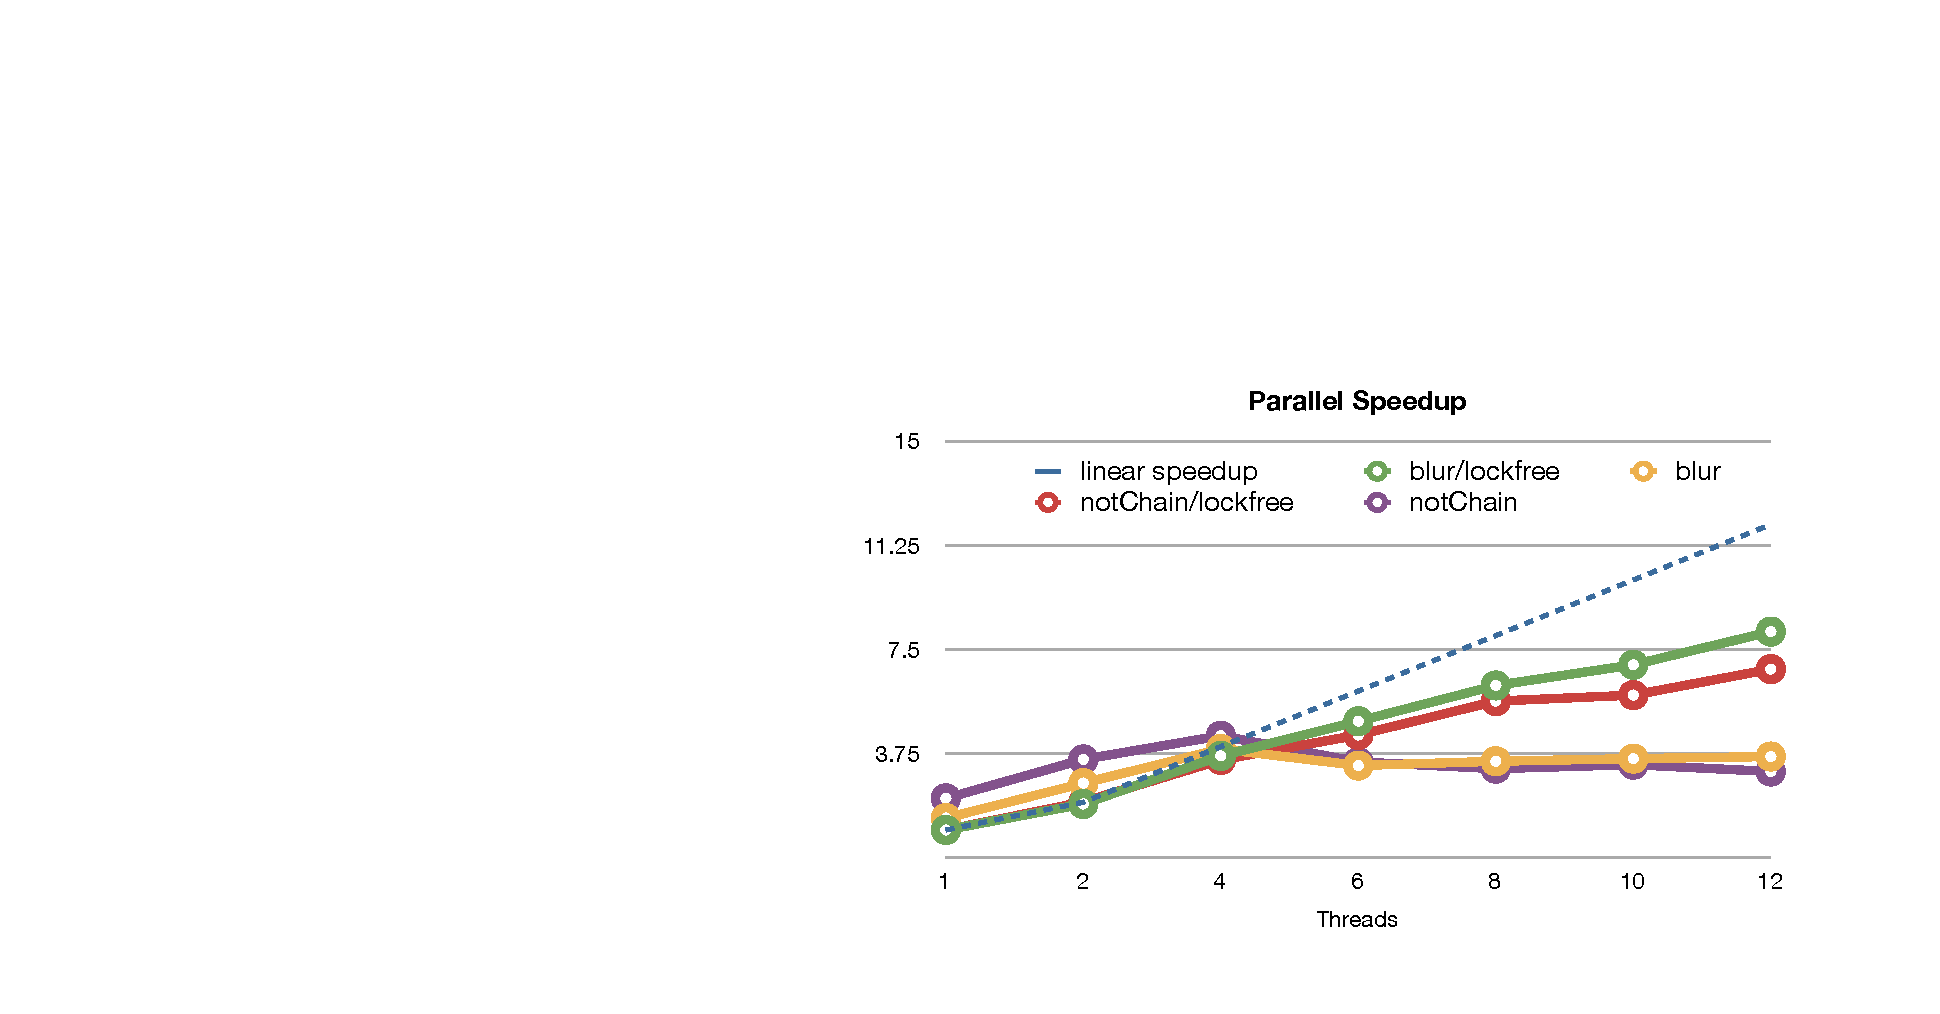
\includegraphics[width=3.3in]{chapter4/figures/CFA_speedups.pdf}
\end{center}
  \caption{Parallel speedup for the ``blur'' and ``notChain'' benchmarks.
    Speedup is normalized to the sequential times for the {\em lock-free}
    versions (5.21s and 9.83s, respectively).  
%
    The normalized speedups are remarkably consistent for the lock-free version
    between the two benchmarks.  But the relationship to the original, purely
    functional version is quite different: at 12 cores, the lock-free LVish
    version of ``blur'' is $202\times$ faster than the original, while ``notChain'' is only
    $1.6\times$ faster, 
    not gaining anything from sharing rather than copying stores
    due to a lack of fan-out in the state graph.
%% which we suspect is due to the lack of optimization in our
%%     skiplist implementation.
}
% \vspace{-4mm}
  \label{fig:bench}
\end{figure}
